\chapter{Introducción}

Este proyecto es de código abierto y está publicado en \href{https://github.com/pabloMillanCb/tfm}{GitHub}, donde se puede acceder al código y documentación íntegros.

\section{Contexto}

\textbf{La industria del videojuego genera más ingresos que la música y el cine juntos}\footnote{\url{https://mediacat.uk/dentsu-gaming-is-bigger-than-music-and-movies-combined/}}. Esta frase tan contundente ha sonado mucho en los últimos años, y no es de extrañar. Lo que antes era percibido como entretenimiento para una demografía infantil y adolescente se ha expandido en las últimas décadas ganando cada vez más presencia en el mercado. Jugar ya no es considerado una cosa solo de niños, y los formatos en los que se pueden encontrar los videojuegos a día de hoy son tan variados como el público que los consume. Se siguen produciendo a juegos de corte clásico para un solo jugador, pero los jóvenes también utilizan juegos con conexión a internet como \textit{Fortnite} como método de socialización fuera de clase. En los transportes públicos pueden verse personas jugando en sus teléfonos móviles experiencias algo más ligeras mientras esperan llegar a su parada. Incluso la tercera edad encontró en \textit{Pokémon Go}, el fenómeno de masas del 2016, una excusa para salir de casa y conocer a otras personas con los mismos intereses. Es muy probable que el lector de este trabajo haya tenido contacto con el mundo del videojuego de una forma u otra, aunque fuera a través del famoso \textit{juego del dinosaurio} que \textit{Google Chrome} muestra cuando no tiene conexión. 

Los videojuegos son productos culturales. Su identidad y las razones de su éxito o fracaso dependen en gran medida de decisiones artísticas y de diseño. Pero, \textbf{los videojuegos antes de nada, son piezas de software} y necesitan de este para existir. Por ello, es de especial interés estudiar y refinar los procesos de ingeniería por los cuales afrontar un desarrollo de estas características. 

En este trabajo, se implementará un videojuego comercial del género \textit{Metroidvania} de principio a fin, poniendo especial interés en el estudio de la metodología de desarrollo.

A continuación se definirán una serie de términos esenciales para el entendimiento del trabajo a realizar.

\begin{itemize}
    \item \textbf{Metroidvania}: Género de videojuegos. El nombre es una combinación de los títulos \textit{Metroid} y \textit{Castlevania}, dos franquicias nacidas a finales de los años 80 que sentaron sus bases. Son juegos basados en la exploración de un gran mapa laberíntico e interconectado donde se deberán sortear pelígros y resolver puzles.

    \item \textbf{Motor de videojuegos}: Un \textit{game engine} o motor de videojuegos es un \textit{framework} especializado en el desarrollo de videojuegos. Entendemos \textit{framework} como una abstracción software con la que, a traves de una serie de herramientas y funcionalidades genéricas, ofrecen un estándar para desarrollar programas de cierta índole, facilitando y acelerando el desarrollo. Estos a menudo están encapsulados en forma de programa o librería. En este trabajo se referirá a los motores de videojuegos simplemente como \textit{motor}.
    
    \item \textbf{Ingeniería del software}: Rama de la informática que estudia los procesos por los cuales diseñar, construir y mantener soluciones basadas en software.

    \item \textbf{Metodologías de desarrollado}: Conjunto de técnicas y métodos organizativos que se aplican para diseñar, implementar y desplegar soluciones software con el objetivo de garantizar la calidad del producto y cumplir los plazos del desarrollo. Son el objeto de estudio de la ingeniería del software.
    
    \item \textbf{Diseño de videojuegos}: Pese a que no hay un consenso en su definición, se puede entender como la labor de diseñar las reglas, contenido, objetivos y visión de un videojuego, bien sea en un marco general (dirigiendo un proyecto entero) o en un área concreta (por ejemplo diseñando los escenarios que recorre el jugador).

\end{itemize} 

\section{Motivación}

\subsection{Industria y proyeccion económica}

El mercado del videojuegos global acumuló un valor de 184 mil millones de dólares en el año 2024 según el reporte anual de \textit{Dentsu}\cite{dentsu-report}, superando al cine y la música, que se posicionan en 33.9 y 28.6 mil millones de dólares respectivamente. En cuanto al panorama español, en la edición de 2023 \textit{Libro blanco de desarrollo español del videojuego}\cite{libro-blanco} se estima que entre el 2022 y el 2026 la facturación nacional de la industria crecerá un 8\%, alcanzando los 1.880 millones.

\begin{figure}[h]
    \centering
    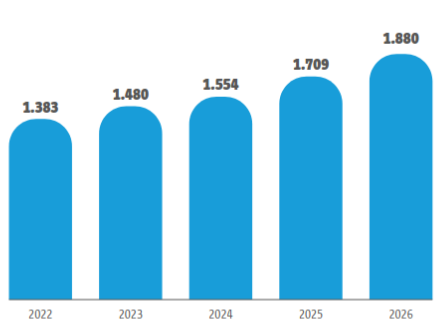
\includegraphics[scale=0.5]{img/prevision_libroblanco.png}
    \caption[Previsión de facturación española de videojuegos]{Previsión de la facturación española de la industria del videojuego en los próximos años según el Libro blanco del desarrollo español de videojuegos 2023}
    \label{fig:prevlibroblanco}
\end{figure}

El interés comercial en desarrollar un producto de valor en esta disciplina se hace evidente ante estos datos.

\subsection{Metodologías de desarrollo}

El software ya es de por si un producto complejo de diseñar, construir o mantener. En el caso de los videojuegos, al ser proyectos de índole creativa se le añaden una serie de características particulares que los diferencian de una aplicación informática genérica.

En primer lugar, un proyecto de software convencional pretende resolver un problema, cubrir una necesidad, o responder a los requisitos de un cliente. Un programa de gestión de agenda, por ejemplo, debe permitir al usuario crear eventos a horas concretas, apuntar tareas pendientes o visualizar un calendario. Estos requisitos pueden ser enumerados y concretados de manera relativamente simple. Ahora bien, ¿cuales son los requisitos de un videojuego? ¿Qué necesidad cubre? En última instancia debe entretener o divertir a un público objetivo. Pero, ¿cómo se especifica eso? ¿Qué elementos debe tener para ser divertido? ¿Cómo se sabe si una idea será divertida antes de invertir tiempo y recursos en implementarla por completo? ¿Cómo se encajan estas cuestiones en el ciclo de desarrollo? Nada de esto evidente desde un principio y añaden difícultades al desarrollo de productos que ya son suficientemente complejos.

Además, al tratarse de proyectos creativos, junto a la programación conviven materias como arte, música y narrativa entre otras. Se cuenta con perfiles tan diversos como artistas conceptuales, modeladores 3D, animadores, compositores, escritories, diseñadores, etc. Todas estas disciplinas se solapan e interconectan unas con otras y dotan de identidad y atractivo al producto final, por lo que es de suma importancia tener en cuenta su gestión en el proceso de desarrollo.

Las grandes producciones del sector (bautizadas como \textit{AAA}) no han hecho más que aumentar en presupuesto y tiempos de desarrollo en los últimos años, llegando a tener algunos proyectos casi una década de duración y cientos de millones de dólares de costo.

\begin{figure}[h]
    \centering
    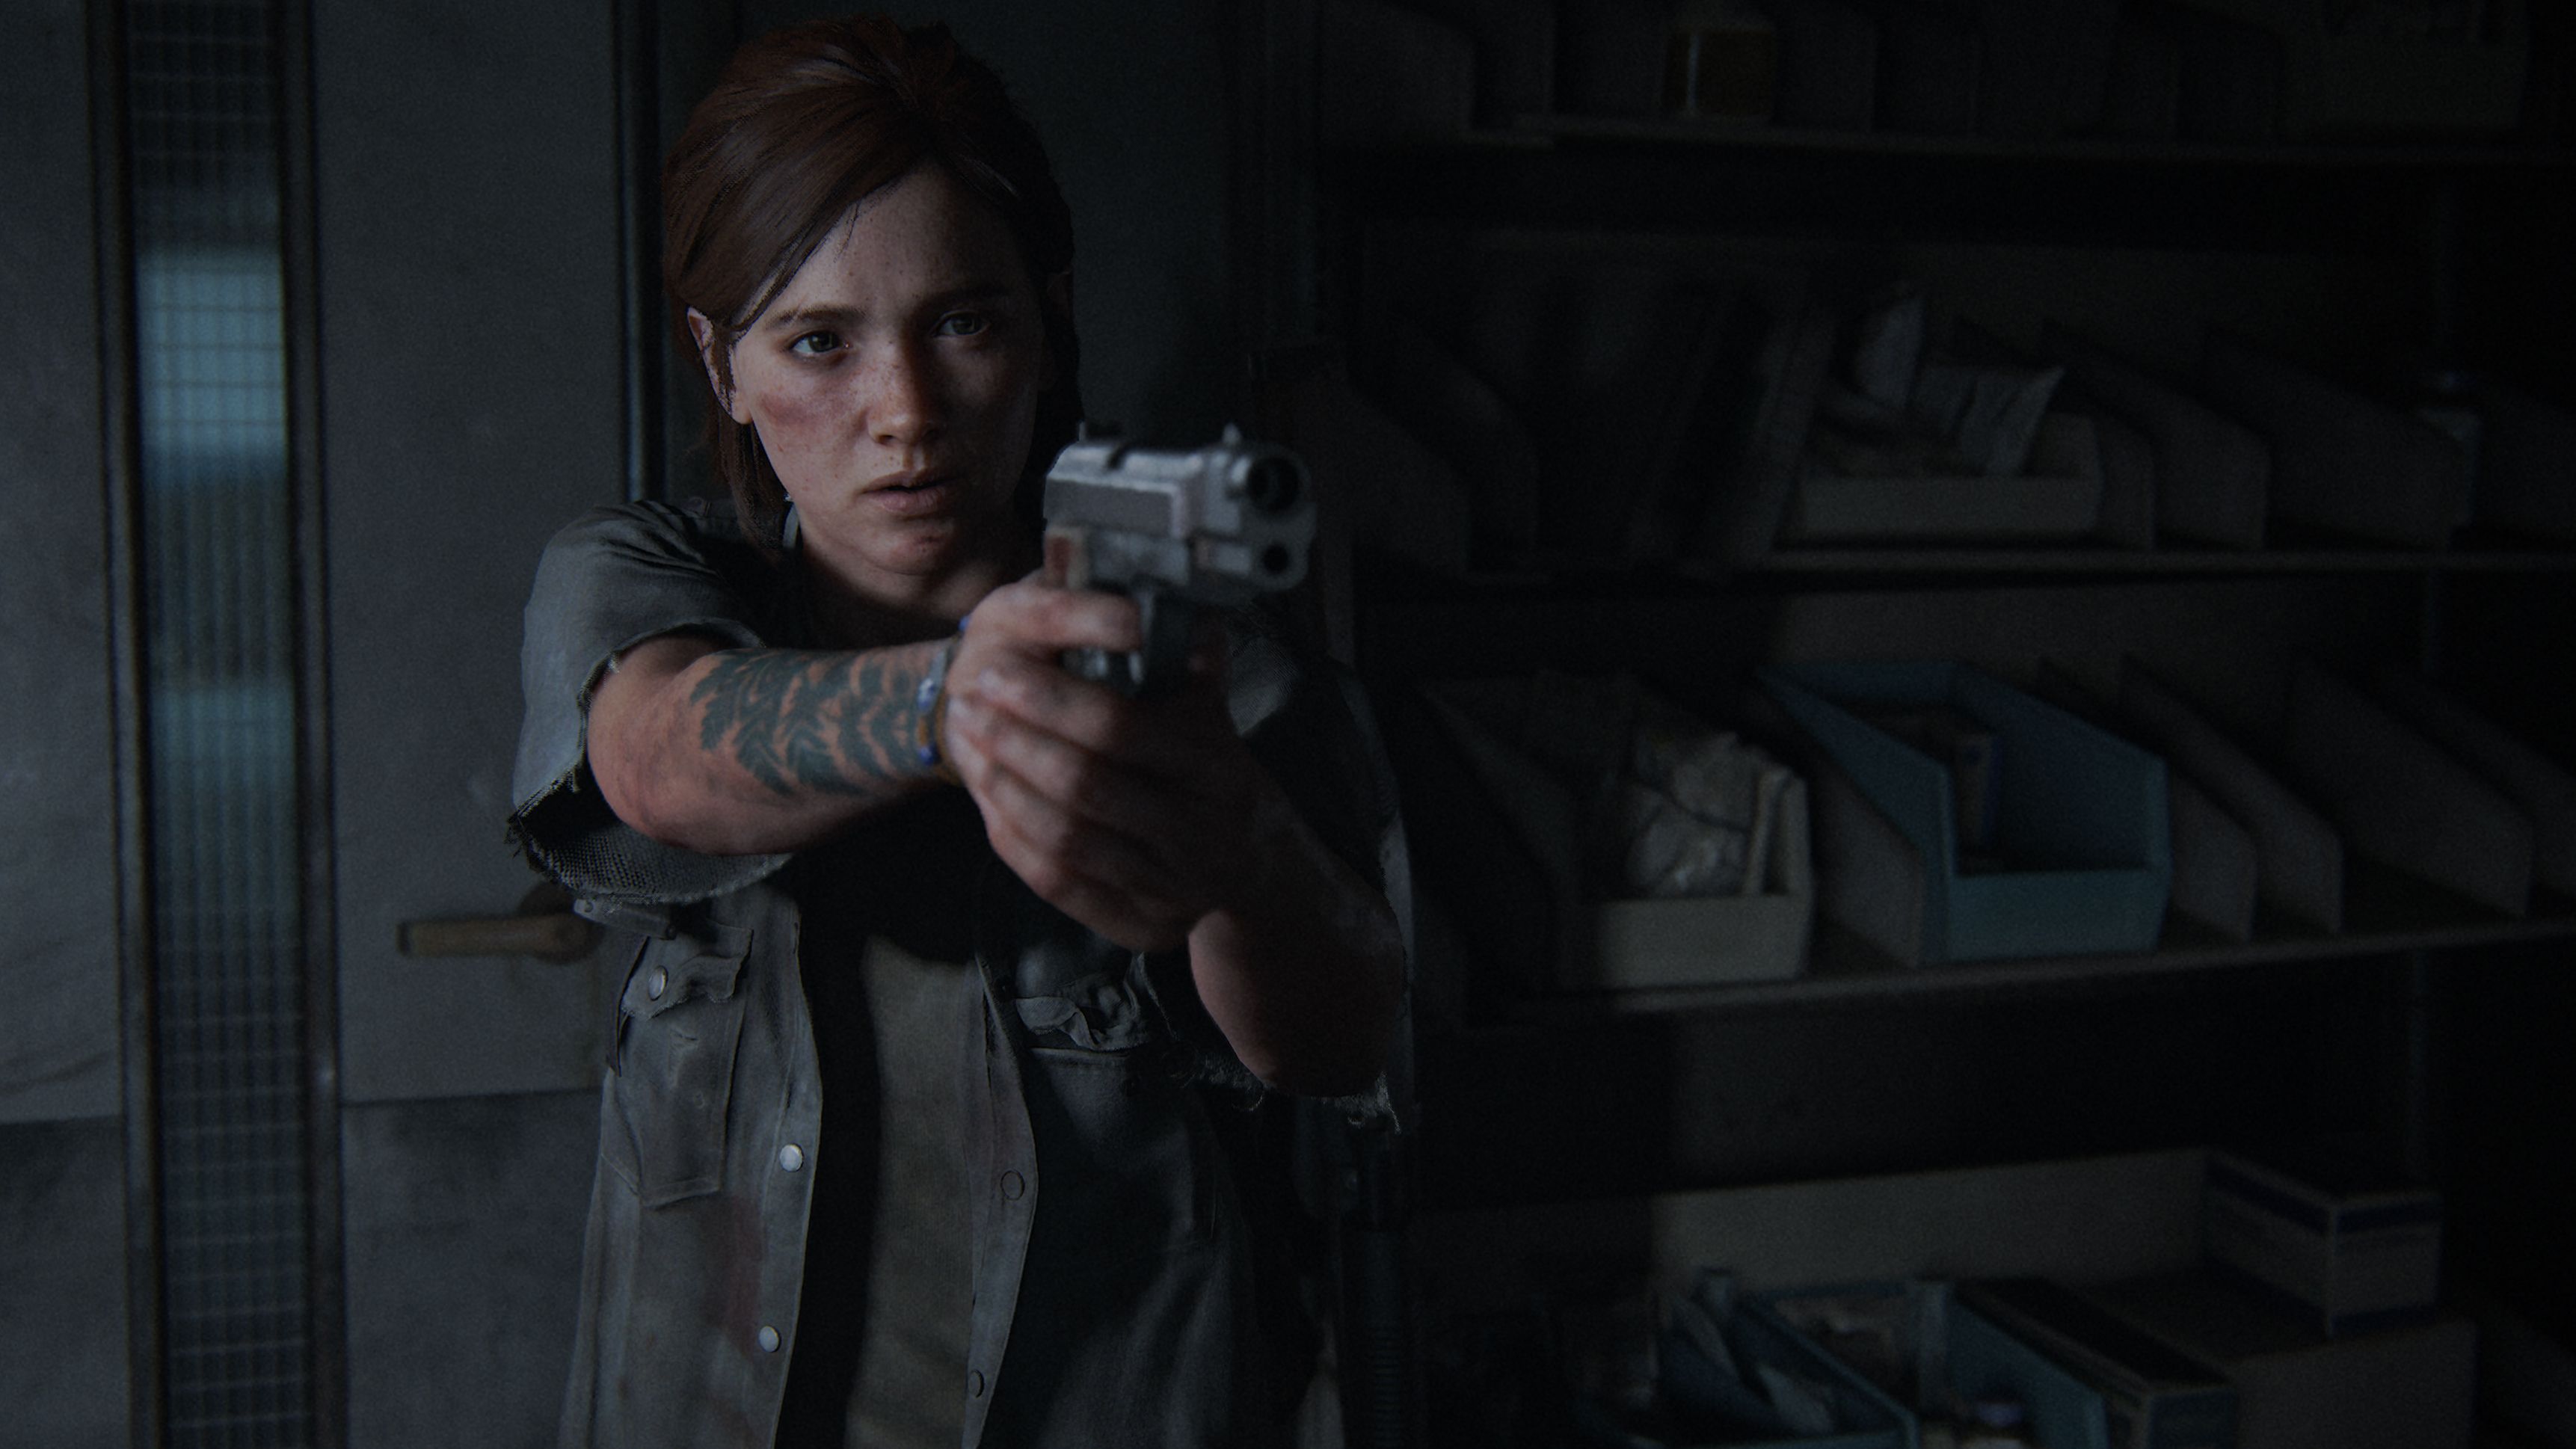
\includegraphics[scale=0.15]{img/tlou.jpg}
    \caption[The Last of Us Parte II]{The Last of Us Parte II, desarrollado por \textit{Naughty Dog}, tuvo un costo de 220 millones de dólares y un desarrollo de 70 meses.}
    \label{fig:tlou2}
\end{figure}

La complejidad software, la naturaleza creativa del diseño lúdico, la multidisciplina y los desarrollos cada vez más ambiciosos son claves para entender por qué a diferencia de otras industrias como la del cine, también con producciones millonarias, los plazos son tan difíciles de cumplir en videojuegos. Hay decenas de ejemplos de retrasos muy sonados, como \textit{The Last Guardian} (Japan Studio), anunciado al público en 2009 con vistas de publicarse en 2011, para finalmente hacerlo en 2016. En un estudio\cite{delayed-games-study} realizado sobre 23,485 juegos lanzados en la plataforma \textit{Steam}, se observó que el 48\% de los proyectos acabaron siendo retrasados respecto a su fecha de lanzamiento anunciada al público.

De esto solo se puede extraer una conclusión: \textbf{el desarrollo de videojuegos tiene necesidades particulares}, no cubiertas por la ingeniería del software genérica, por lo que es de especial interes estudiar y adaptar los procesos de desarrollo para cubrir estas necesidades.

\subsection{Tecnologías y sistemas específicos}

Existen multitud de técnicas y tecnologías que se pueden aplicar a un videojuego para enriquecer la experiencia del jugador. Por ejemplo los \textit{shaders}, programas especializados que hacen uso del hardware de las \textit{GPUs} para generar efectos gráficos avanzados con un coste computacional muy bajo.

Por otro lado, como ya se estableció previamente, los \textit{Metroidvania} tratan sobre la exploración de un enorme y laberíntico mapa. Para hacer de esto una tarea divertida para el jugador, se necesitan implementar sistemas e interfaces de mapeado, a través de las cuales orientarse y llevar la cuenta de qué sitios se ha visitado y cuales no. Sería interesante que interfaces contaran con un sistema de navegación asistida que haga uso de técnicas inteligentes de pathfinding para indicar al jugador la ruta entre dos puntos del mapa.

El jugador rara vez se encuentra solo en juegos del género. El mundo está habitado por NPC (\textit{Non-playable characters}), personajes que no controla el jugador. Estos pueden ser tanto amistosos como hostiles, y para ello se les debe dotar de cierto comportamiento. Esto se puede lograr implementando un sistema de gestión para el comportamiento de NPCs, con el que a partir de ciertos parámetros el desarrollador pueda configurarlos fácilmente, acelerando en el largo plazo el proceso de desarrollo.


\section{Objetivos}

El objetivo principal de este trabajo será desarrollar un videojuego de género \textit{Metroidvania} empleando el motor \textit{Godot}. El resultado será un producto completo de principio a fin, integrando todos los ámbitos del desarrollo a parte del técnico como el arte, sonido y diseño. Este objetivo se desgrana en los siguientes objetivos específicos:

\begin{itemize}
    \item \textbf{OE1}: Estudio y aplicación de metodologías de desarrollo y testeo de videojuegos para asegurar un producto de calidad, ajustándose a las necesidades específicas de este tipo de software.
    \item \textbf{OE2}: Estudio y aplicación de patrones, arquitecturas y convenciones del motor Godot para producir un código mantenible en el tiempo y un buen rendimiento del juego en tiempo de ejecución.
    \item \textbf{OE3}: Implementación de los sistemas y módulos necesarios para realizar un juego \textit{Metroidvania} como un menú de mapas dinámico, registro de zonas exploradas, sistema de cálculo de rutas por pathfinding y un sistema de comportamiento para NPC (non-player characters).
    \item \textbf{OE4}: Desarrollo y aplicación de \textit{shaders} para lograr efectos visuales llamativos.

\end{itemize} 

\section{Estructura de la memoria}

//to do